%!TEX TS-program = xelatex
\documentclass[]{friggeri-cv}
\usepackage{afterpage}
\usepackage{hyperref}
\usepackage{color}
\usepackage{xcolor}
\usepackage{smartdiagram}
\usepackage{fontspec}
% if you want to add fontawesome package
% you need to compile the tex file with LuaLaTeX
% References:
%   http://texdoc.net/texmf-dist/doc/latex/fontawesome/fontawesome.pdf
%   https://www.ctan.org/tex-archive/fonts/fontawesome?lang=en
%\usepackage{fontawesome}
\usepackage{metalogo}
\usepackage{dtklogos}
\usepackage[utf8]{inputenc}
\usepackage{tikz}
\usetikzlibrary{mindmap,shadows}
\hypersetup{
    pdftitle={},
    pdfauthor={},
    pdfsubject={},
    pdfkeywords={},
    colorlinks=false,           % no lik border color
    allbordercolors=white       % white border color for all
}
\smartdiagramset{
    bubble center node font = \footnotesize,
    bubble node font = \footnotesize,
    % specifies the minimum size of the bubble center node
    bubble center node size = 0.5cm,
    %  specifies the minimum size of the bubbles
    bubble node size = 0.5cm,
    % specifies which is the distance among the bubble center node and the other bubbles
    distance center/other bubbles = 0.3cm,
    % sets the distance from the text to the border of the bubble center node
    distance text center bubble = 0.5cm,
    % set center bubble color
    bubble center node color = pblue,
    % define the list of colors usable in the diagram
    set color list = {lightgray, materialcyan, orange, green, materialorange, materialteal, materialamber, materialindigo, materialgreen, materiallime},
    % sets the opacity at which the bubbles are shown
    bubble fill opacity = 0.6,
    % sets the opacity at which the bubble text is shown
    bubble text opacity = 0.5,
}

\addbibresource{bibliography.bib}
\RequirePackage{xcolor}
\definecolor{pblue}{HTML}{0395DE}

\begin{document}
\header{Satheesh}{Charles}
      {DevOps Engineer}
      
% Fake text to add separator      
\fcolorbox{white}{gray}{\parbox{\dimexpr\textwidth-2\fboxsep-2\fboxrule}{%
.....
}}

% In the aside, each new line forces a line break
\begin{aside}
  
\includegraphics[scale=0.30]{img/Satt.jpg}
  %\section{Address}
  %  Chennai
   % India
   % ~
  \section{Mob \& Skype}
    +852 5427 5754
    satheesh.charles
    ~
  \section{Mail}
    \href{mailto:satheesh.charles@gmail.com}{\textbf{satheesh.charles@}\\gmail.com}
    ~
    \section{GitHub}
    \href{https://github.com/satheeshCharles}{satheeshCharles}
    ~
  \section{Web \& linked-in}
    \href{https://www.linkedin.com/in/satheesh-charles/}{satheesh charles}
    %\href{https://bitbucket.org/mygit}{bitbucket.org/mygit}
    %\href{https://github.com/mygit}{github.com/mygit}
    %\href{https://gitlab.com/u/mygit}{gitlab.com/u/mygit}
    ~
    ~
    ~
  % use  \hspace{} or \vspace{} to change bubble size, if needed
  \section{Contribution}
    \smartdiagram[bubble diagram]{
        \textbf{DevOps},
        \textbf{Jenkins}\\\textbf{},
       % \textbf{Python},
        \textbf{OS},
        \textbf{Puppet},
        \textbf{Others\vspace{3mm}},
        \textbf{Nomad},
        \textbf{Vault},
        \textbf{Shell},
        \textbf{Docker}
    }
    ~
  \section{Personal Skills}
    \smartdiagram[bubble diagram]{
        \textbf{Team}\\\textbf{Player},
        \textbf{Initiative},
        \textbf{Curiosity},
        \textbf{Problem}\\\textbf{Solving},
        \textbf{\vspace{2mm}Manage\vspace{2mm}},
        \textbf{Organize}
    }
    ~
\end{aside}
~

\section{tl;dr}
\begin{entrylist}
  \entry
    {}
    {}
   {}
  {11 + years of experience. Loves to understand,build and operate Devops distributed systems.Technology enthusiast. Brings a Bachelor’s Degree in Computers and master degree in information systems. }
\end{entrylist} 


\section{Experience}
\begin{entrylist}
  \entry
    {11/18 - Now}
    {DevOps Engineer}
    {M800}
    {Creating secured application flow with Vault and Consul. Have providing engineering support for the CI/CD and containerized ecosystem.}
  \entry
    {12/10 - 11/18}
    {DevOps Engineer}
    {Bank of NewYork Mellon}
    {Researched, developed and implemented Jenkins,Puppet and Docker infrastructure. Worked on various micro services. Instrumented automatic scaling processes by Nomad on BNY cloud. Implemented various monitoring methods into deployment processes to develop self-healing solutions. Automated varied BAU tasks by scripting. }
  \entry
    {06/07 - 11/10}
    {Java Developer and Middleware Consultant}
    {Satyam Computer Services}
    {Have experience in Development Designing Architectural and solutions in Java and Middleware Products. Worked in various environments and tuning for optimal performance. Automated job manager tasks by scripting. Involved in MQ engineering support tasks}
   
   
\end{entrylist}
    %{06/07 - 06/08}
    %{Enter Lelvel technology Programmer}
    %{Satyam Computer Services}
    %{Web development experience and Evaluate Serena Dimension for Java component migration.  }


\section{Skills}
\begin{entrylist}
 \entry
    { }
    {DevOps}
    {}
    {Jenkins, Docker, Vault, Consul, Nomad, Puppet, MCO, Basic Linux Administration, Confluence and  Jira }
 \entry
    { }
    {Automation \& Middle-ware}
    {}
    {Shell, Python, Apache, Tomcat ,WebSphere Application Server}

%  \entry
%    {2005 - 2009}
%    {Bachelor's Degree in Computer Engineering}
%    {School}
%    {Lorem ipsum dolor sit amet, consectetur adipiscing elit, sed do eiusmod tempor incididunt ut labore et dolore magna aliqua. Ut enim ad minim veniam, quis nostrud exercitation ullamco laboris nisi ut aliquip ex ea commodo consequat\\}
%  \entry
%    {2000 - 2005}
%    {Scientific Disploma}
%   {School}
%    {Lorem ipsum dolor sit amet, consectetur adipiscing elit, sed do eiusmod tempor incididunt ut labore et dolore magna aliqua}
\end{entrylist}
\section{Certifications}
\begin{entrylist}
  \entry
    {11/2017}
    {Block Chain Essentials}
    {IBM}
    {}
    %{Lorem ipsum.\\
    %\emph{Lorem ipsum}}
    \entry
    {11/2013}
    {IBM WebSphere Application Server Network Deployment V7.0}
    {IBM}
    {}
    \entry
    {13/2009}
    {Sun Certified Java Programmer}
    {SUN}
    {}
\end{entrylist}

%\newpage

%\begin{aside}
 % \section{OS Preference}
 %   \textbf{Linux}
\includegraphics[scale=0.40]{img/5stars.png}
 %   \textbf{Unix}
\includegraphics[scale=0.40]{img/4stars.png}
 %   \textbf{MacOS}
\includegraphics[scale=0.40]{img/2stars.png}
 %   \textbf{Windows}
\includegraphics[scale=0.40]{img/1stars.png}
    ~
  %\section{Places Lived}
    %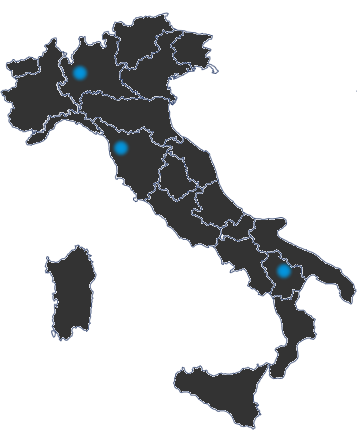
\includegraphics[scale=0.25]{img/italia.png}
    ~
  %\section{Languages}
   % \textbf{Italian}
\includegraphics[scale=0.40]{img/5stars.png}
   % \textbf{English}
\includegraphics[scale=0.40]{img/4stars.png}
    ~
%\end{aside}

%\section{Publications}
%Author, Author, Author\\
%\textbf{Lorem ipsum dolor sit amet, consectetur adipiscing elit, sed do eiusmod tempor incididunt ut labore et dolore magna aliqua}\\
%\emph{Lorem ipsum dolor sit amet, consectetur adipiscing elit, sed do eiusmod tempor incididunt ut labore et dolore magna aliqua}
%\\
%\section{Certifications}
%\begin{entrylist}
%  \entry
 %   {11/2017}
 %   {Block Chain Essentials}
%    {IBM}
 %   {}
 %   %{Lorem ipsum.\\
    %\emph{Lorem ipsum}}
%\end{entrylist}



%\begin{flushleft}
%emph{May 8th, 2016}
%\end{flushleft}
\begin{flushright}
\footnotesize{Satheesh Charles}
\end{flushright}
%\monthyeardate\today

\end{document}
